\subsubsection{Experiments for Eliciting Sad Emotion}

To capture sad emotional responses at different intensities, three distinct tasks were designed. These tasks use music and emotionally powerful videos, which are known to effectively evoke sadness through auditory and visual pathways.

\paragraph*{Low-Intensity Sadness – Listening to “Little Motel” by Modest Mouse}

The first task involves participants listening to the song “Little Motel” by Modest Mouse \url{https://youtu.be/zqQTODR3kR8?si=yqNkeWlbUYPNUEXb} \citep{modest_mouse_little_motel}, accompanied by a short explanation highlighting the lyrical themes of heartbreak, regret, and emotional distance. Sad music has been shown to be an effective tool for inducing low-level sadness, although the emotional response may include feelings of nostalgia, aesthetic pleasure, or being emotionally moved~\citep{ribeiro2019emotional}.

“Little Motel” is commonly described by listeners as emotionally evocative and melancholic, largely due to its subdued instrumentation and reflective lyrics. Anecdotal listener feedback, such as that found in public forums~\cite{redditLittleMotel}, reinforces this emotional interpretation. Providing context before playing the song helps guide participants' emotional attention, making the sadness more focused and easier to observe.

\paragraph*{Medium-Intensity Sadness – Viewing a Clip of a Young Person in Distress}

For medium-intensity sadness, participants were shown a video clip of a young person crying while overwhelmed by everyday struggles. Research supports the use of video stimuli for eliciting sadness, particularly when they depict realistic, relatable struggles and human vulnerability. Visual and auditory cues together create a more immersive emotional experience compared to music or images alone~\citep{nojavanasghari2016emoreact}.

Scenes involving children or youth in distress can be especially powerful due to their perceived innocence and relatability, increasing empathy from the viewer. As a result, this type of content tends to generate a moderate level of sadness while remaining emotionally grounded.

\paragraph*{High-Intensity Sadness – "The Champ" (1979) Death Scene}

The third task used a well-known emotionally intense video: the final scene from the 1979 film "The Champ", in which a young boy reacts to the death of his father (\url{https://youtu.be/b5qwTeCj4jc?si=2HJe3G0KL6U6azXY}) \citep{luiza_lootens_champ_final}. This particular clip is considered a gold standard in emotion research for eliciting high-intensity sadness. It has been cited in numerous studies, including foundational work by Gross and Levenson (1995), and appears in validated databases like E-MOVIE~\citep{kuijsters2016inducing, maffei2019movie}.

The scene evokes intense grief and helplessness, making it a powerful tool for eliciting high levels of sadness. Its use in many research studies confirms its reliability and emotional impact across different participant groups.

Figure~\ref{fig:task-sad} shows the screenshots related to the sadness eliciting tasks.

\begin{figure*}[h]
    \centering
    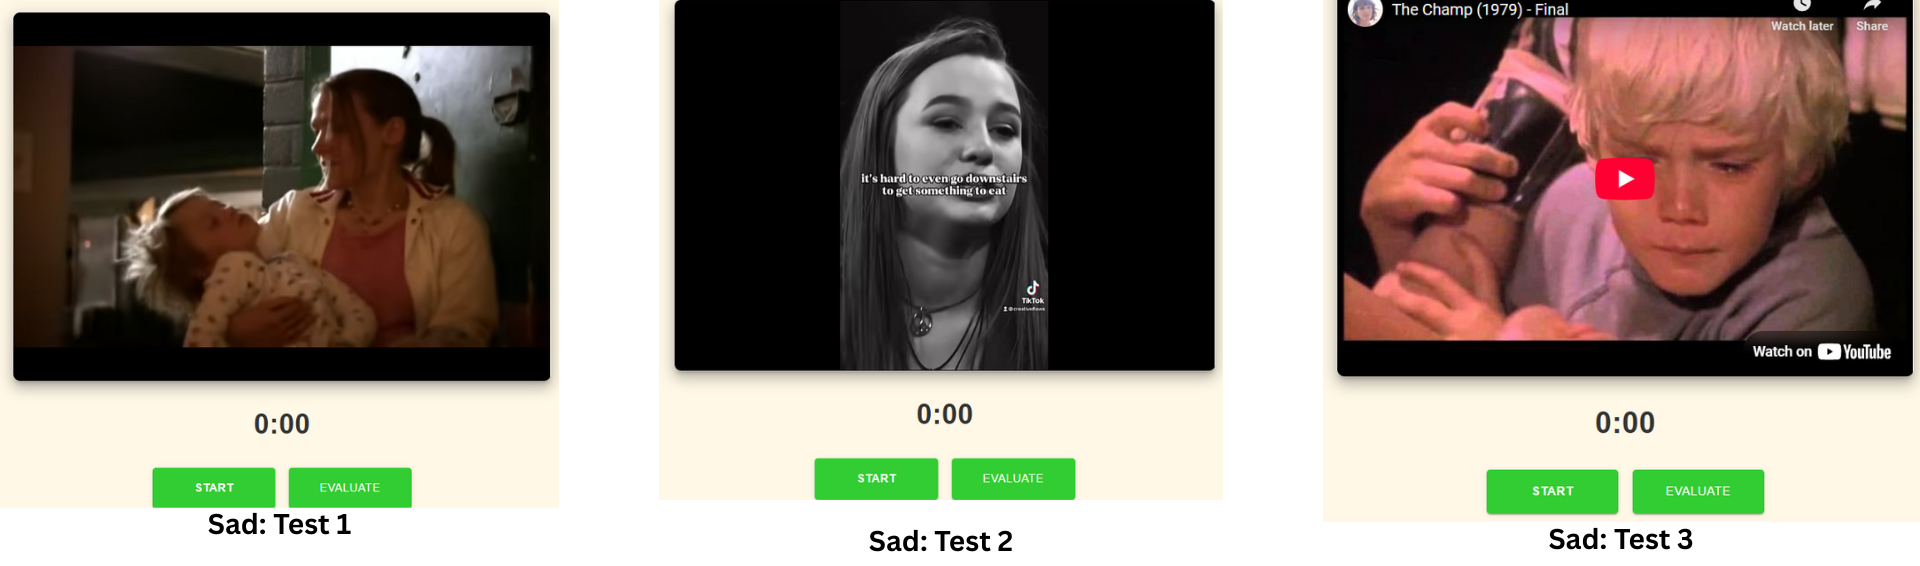
\includegraphics[width=1\textwidth]{img/chapter_03/sad_tests.png}
    \captionof{figure}{Eliciting tasks for Sad Emotion}
    \label{fig:task-sad}
\end{figure*}